\documentclass{standalone}
\usepackage{tikz-network}
\begin{document}
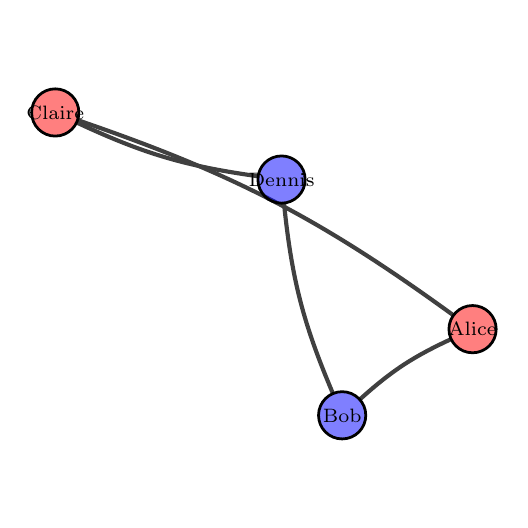
\begin{tikzpicture}
\clip (0,0) rectangle (6,6);
\Vertex[x=5.650,y=2.171,color=red,opacity=0.5,label=Alice]{a}
\Vertex[x=3.994,y=1.077,color=blue,opacity=0.5,label=Bob]{b}
\Vertex[x=0.350,y=4.923,color=red,opacity=0.5,label=Claire]{c}
\Vertex[x=3.224,y=4.071,color=blue,opacity=0.5,label=Dennis]{d}
\Edge[,bend=-8.531](a)(b)
\Edge[,bend=-8.531](a)(c)
\Edge[,bend=-8.531](c)(d)
\Edge[,bend=-8.531](d)(b)
\end{tikzpicture}
\end{document}